\documentclass[11pt,a4paper]{article}
\usepackage[utf8]{inputenc}
\usepackage[english]{babel}
\usepackage{hyperref}
\usepackage{url}
\usepackage{graphicx}
\usepackage{subfig}
\usepackage{pdfpages}

\title{%
    \textbf{R \& D Workshop} \\
    Tomcat in the Cloud \\
    \\
    \textbf{Initial Plan}
}

\author{%
    Ismaïl Senhaji \\
    \small \href{mailto:ismail.senhaji@unifr.ch}{ismail.senhaji@unifr.ch} \\
    \\
    Guillaume Pythoud \\
    \small \href{mailto:guillaume.pythoud@unifr.ch}{guillaume.pythoud@unifr.ch}
    \\
    \\
    Supervised by \\
    Jean-Frederic Clere \\
    \small \href{mailto:jclere@redhat.com}{jclere@redhat.com}
}

\date{March 26, 2017}

\begin{document}
\graphicspath{{fig/}}

\maketitle

\begin{figure}[b]
    \centering
    \subfloat{
\includegraphics[height=1.5cm]{jmcs.png}}
    \\
    \subfloat{
\includegraphics[height=1.6cm]{redhat-logo.png}}
\end{figure}

\newpage
\tableofcontents

\newpage


\section{Project description}

\subsection{Project and context}

For this project, we have been assigned to \emph{Red
    Hat}~\footnote{http://www.redhat.com/en/about}. Red Hat is an international
software and company, specializing in open source.  Among others, they develop
the \emph{OpenShift Container
    Platform}~\footnote{https://www.openshift.com/container-platform/index.html},
which is full-stack cloud management solution.

We will work on the
\emph{Tomcat}~\footnote{https://www.openshift.com/container-platform/index.html}
Java web server. Our task is to extend Tomcat in order to make session
replication work in a cloud environment.

As it stands, session replication in Tomcat is not cloud ready yet. The main
issue is that it uses multicast which only works in a local network. In a cloud
deployment, instances can be distributed over the internet. This calls for the
development of a new session replication solution.


\subsection{Goals and objectives of the project}

The major goal of the project to make Tomcat's session work in the cloud. This
goal is divided in 3 steps:
\begin{enumerate}
    \item Study existing methods
    \item Implement a new solution based on one of those methods
    \item Test the implementation
\end{enumerate}

To test our implementation, we will develop a very Java web application. It
will simply display these informations:

\begin{itemize}
    \item The ID of the Tomcat instance that served the request
    \item The user's session ID
    \item A counter that is incremented on every request.
\end{itemize}

A secondary goal is to build and configure a Raspberry Pi cluster, running
OpenShift. If successful, it will be presented as a demonstration at the end of
the project.

Another important goal is to provide detailed documentation for future users.
We will write a ``Quick Start Guide'' detailing the steps to follow to have a
working Tomcat cluster running in an OpenShift cloud.


\section{Project organisation}

We are working on this project as a team of two. We plan on reserving two days
per week to work exclusively on this projects, and will aim to meet at least
once a week to discuss issues and synchronize our efforts. All development will
take place on the GitHub
repository~\footnote{https://www.openshift.com/container-platform/index.html}
we set up for this project. The repository's wiki contains a logbook that will
periodically be updated during the project.

\subsection{Responsibility distribution}

\begin{itemize}
    \item Ismaïl Senhaji, Student \\
        \href{mailto:ismail.senhaji@unifr.ch}{ismail.senhaji@unifr.ch}
    \item Guillaume Pythoud, Student \\
        \href{mailto:guillaume.pythoud@unifr.ch}{guillaume.pythoud@unifr.ch}
    \item Jean-Frédéric Clere, Project supervisor at Red Hat \\
        \href{mailto: jclere@redhat.com}{jclere@redhat.com}
    \item Dr.\ Hughes Mercier, Workshop coordinator \\
        \href{mailto: hugues.mercier@gmail.com}{hugues.mercier@gmail.com}
\end{itemize}

\subsection{Interactions with the client}

Communication with Jean-Frederic Clere is done mainly via e-mail. As the Red
Hat office is located in Neuchâtel, we also have the possibility to meet there
in person to discuss things more thoroughly, and in fact we have already done
so twice.

Jean-Frederic Clere has been given access to our GitHub repository and can
monitor our progress.

\section{Methodology}

Most development will be done in Java, since Tomcat itself is written in Java.
But we suspect that most time will be spent on reading documentation and code
than on writing code.

As mentioned above, all our work is available on our GitHub repository, be it
code, documentation or simply comments and ideas.

For testing our solutions, we will use
MiniShift~\footnote{https://www.openshift.org/minishift/}. MiniShift is a tool
that deploys a ``local'' (i.e.\ consisting of a unique machine) OpenShift
cluster on any computer. This will allow us run tests on our laptops, saving
the time necessary to deploy a real OpenShift installation. Only towards the
end of the project, when everything else is done, will we finally deploy our
solution on a real cluster.

\subsection{State of the art}

Our research has shown that Tomcat has two built-in session replication
solutions that could be built
on\footnote{https://tomcat.apache.org/tomcat-8.5-doc/cluster-howto.html}:

\begin{enumerate}
    \item \emph{DeltaManager}: this session manager replicates session data to
        all other instances in a cluster. Peer discovery can be either be done
        statically or dynamically. In static mode, a list of peers is hardcoded
        in Tomcat's configuration file. In dynamic mode, peers are discovered
        using multicast.

    \item \emph{PeristanceManager}: session data is stored in the filesystem or
        in a JDBC-capable database.
\end{enumerate}

Paths to explore are modifying DeltaManager to discover peer using a different
method (since multicast over the internet isn't feasible), or configure
PersistanceManager to use a distributed datastore. The first solution might be
more interesting from a performance point of view.

Finally, if none of the solutions above turn out fruitful, there still are
other paths to explore: there are solutions that bypass Tomcat's session
manager and use an external one instead. The \emph{Spring
    Framework}~\footnote{http://projects.spring.io/spring-framework/} offers
such a solution, and is advertised to have built-in support for distributed
datastores such as \emph{Redis} or
\emph{Hazelcast}\footnote{http://docs.spring.io/spring-session/docs/current/reference/html5/}.
Another solution ports WildFly's session manager to
Tomcat\footnote{https://github.com/wildfly-clustering/wildfly-clustering-tomcat}.

While these solutions using external session managers are known to work, we
will mainly concentrate on those based on Tomcat, as they avoid relying on too
many external dependencies. But we consider them as a ``Plan B'' if all else
fails.

\section{Constraints and elements of risk}

In this projects, we face two major risks:

The first is getting lost in the complexity of the Tomcat and OpenShift
ecosystems. Fortunately, these projects are usually well-documented. The open
source community is also very helpful: we can find support on discussion forums
and IRC chatrooms. And since the projects are open source, we can study the
source code to gain insight on its inner workings.

The second risk is not being able to produce a working solution in time. Our
main target is to develop a solution based on DeltaManager of
PersistanceManager as explained above. If this turns out to be too
time-consuming, technically difficult, or plain impossible, we will fall back
to ``Plan B'' (using an external session manager). We will make this choice
before the midterm presentation.

In case we opt for this fallback solution, we
will document the reason for our failures, in the hope that these pitfalls
might be avoided by someone attempting the same task in the future.

Furthermore, if we fall behind our schedule, we can cancel installing a
Raspberry Pi cluster, as this is not a hard requirement.

\section{Deliverable goods}

At the end of this project we will deliver the following items:

\begin{enumerate}
    \item A simple Java Web Application to test session replication
    \item Source code of our modifications to the Tomcat server
    \item Documentation in the form of a ``Quick Start Guide'', explaining how
        to easily run Tomcat using our modifications on an OpenShift cloud
    \item (optional) A working demonstration of our work running on a Raspberry
        Pi cluster.
\end{enumerate}

Items 1--3 will be available on our GitHub repository, item 4 will be presented
during the final presentation.

\section{Efforts and schedule}

Our workplan is available on our GitHub
repository\footnote{https://github.com/iSma/tomcat-in-the-cloud/wiki/Workplan}
and is reproduced in figure~\ref{fig:workplan}.

\begin{figure}[H]
    \centering
    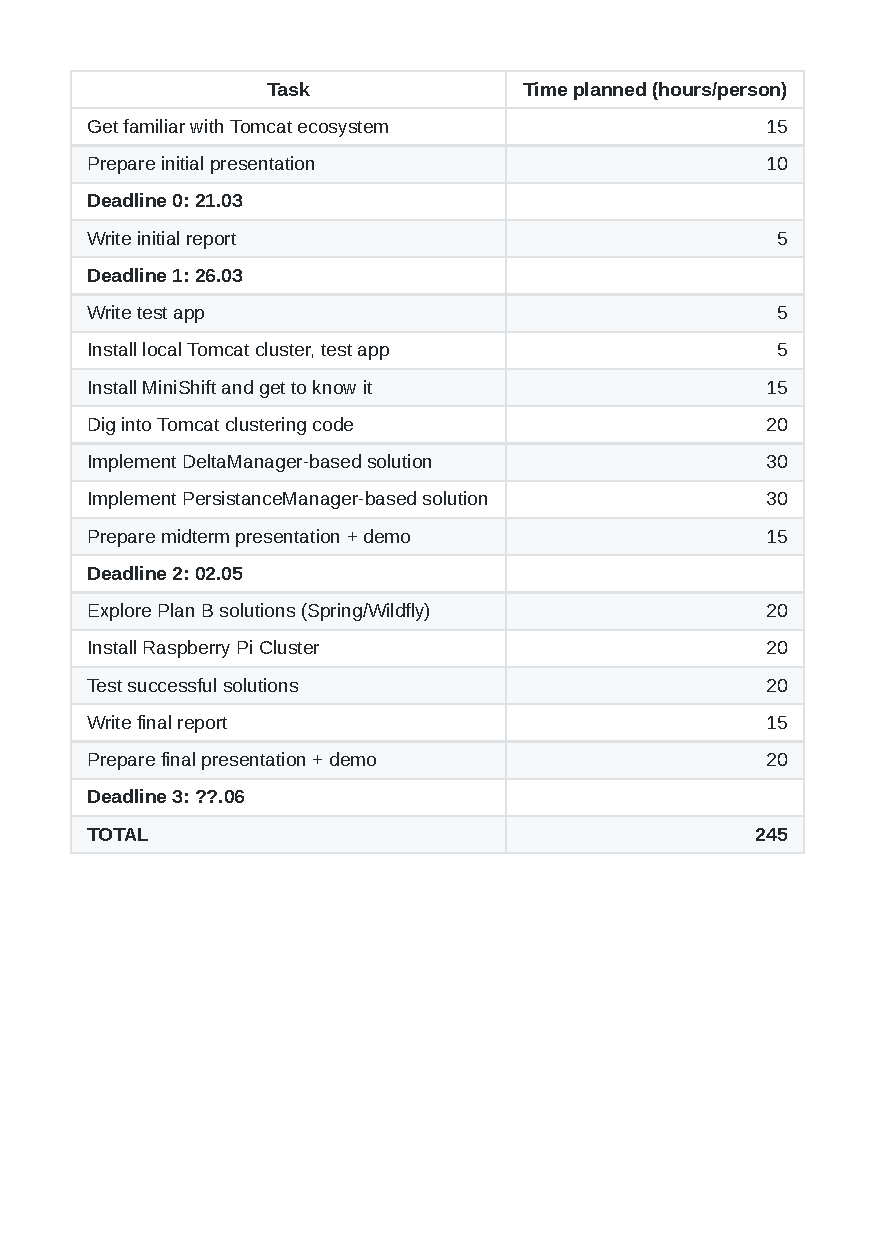
\includegraphics[trim=400 150 400 0]{workplan}
    \caption{Workplan}\label{fig:workplan}
\end{figure}

\end{document}
